

\documentclass[journal,transmag]{IEEEtran}
\hyphenation{op-tical net-works semi-conduc-tor}

\usepackage{enumitem}

% *** GRAPHICS RELATED PACKAGES ***
%
\ifCLASSINFOpdf
   \usepackage[pdftex]{graphicx}
  % declare the path(s) where your graphic files are
  % \graphicspath{{../pdf/}{../jpeg/}}
  % and their extensions so you won't have to specify these with
  % every instance of \includegraphics
  % \DeclareGraphicsExtensions{.pdf,.jpeg,.png}
\else
  % or other class option (dvipsone, dvipdf, if not using dvips). graphicx
  % will default to the driver specified in the system graphics.cfg if no
  % driver is specified.
  % \usepackage[dvips]{graphicx}
  % declare the path(s) where your graphic files are
  % \graphicspath{{../eps/}}
  % and their extensions so you won't have to specify these with
  % every instance of \includegraphics
  % \DeclareGraphicsExtensions{.eps}
\fi
% graphicx was written by David Carlisle and Sebastian Rahtz. It is
% required if you want graphics, photos, etc. graphicx.sty is already
% installed on most LaTeX systems. The latest version and documentation
% can be obtained at: 
% http://www.ctan.org/pkg/graphicx
% Another good source of documentation is "Using Imported Graphics in
% LaTeX2e" by Keith Reckdahl which can be found at:
% http://www.ctan.org/pkg/epslatex
%
% latex, and pdflatex in dvi mode, support graphics in encapsulated
% postscript (.eps) format. pdflatex in pdf mode supports graphics
% in .pdf, .jpeg, .png and .mps (metapost) formats. Users should ensure
% that all non-photo figures use a vector format (.eps, .pdf, .mps) and
% not a bitmapped formats (.jpeg, .png). The IEEE frowns on bitmapped formats
% which can result in "jaggedy"/blurry rendering of lines and letters as
% well as large increases in file sizes.
%
% You can find documentation about the pdfTeX application at:
% http://www.tug.org/applications/pdftex





\begin{document}

\title{\textsc{Gases Ideales}}

\author{
\IEEEauthorblockN{David S. Castro , William A. Gómez,  Ana M. Niño, Laura V. Pachón , Juliana Ramos y Luis A. Cañón,}
\IEEEauthorblockA{Pontificia Universidad Javeriana, Bogotá, Colombia}
\IEEEauthorblockA{Informe de laboratorio de Gases Ideales}
\IEEEauthorblockA{Grupo I}

}
% The paper headers
\markboth{Gases Ideales. Octubre 28~2021}%
{Shell \MakeLowercase{\textit{et al.}}: Bare Demo of IEEEtran.cls for IEEE Transactions on Magnetics Journals}
\IEEEtitleabstractindextext{%

	\begin{abstract}
	This laboratory report aims to analyze the behavior of an ideal gas, taking into account its state equation and the different processes that make it up. For this purpose, we made use of the PHET simulator which allowed us to work with an ideal gas and its different properties, in order to study the variables of pressure, volume and temperature in four different cases: the first with a constant volume, the second with a constant temperature, the third with a constant pressure as a function of temperature and the other as a function of volume, and as a fourth case were all the variable factors making changes in the size of the container. Finally, a collection of the data obtained for each of the cases was carried out, in order to plot them and determine their behavior. 
	\end{abstract}
	\begin{IEEEkeywords}
	 Law of gases, equation of state, processes with ideal gases, pressure, volume, temperature. 
	 	\end{IEEEkeywords}}


\maketitle
\IEEEdisplaynontitleabstractindextext
\IEEEpeerreviewmaketitle


\section{Resumen}

En el presente informe de laboratorio se pretende analizar el comportamiento de un gas ideal, teniendo en cuenta su ecuación de estado y los diferentes procesos que lo conforman. Para esto se hizo uso del simulador PHET el cual nos permitió trabajar con un gas ideal y sus diferentes propiedades, para así estudiar las variables de presión, volumen y temperatura en cuatro casos diferentes: el primero con un volumen constante, el segundo con temperatura constante, el tercero con presión constante mostrado en función de la temperatura y otra en función del volumen, y como cuarto caso se encontraban todos los factores variables realizando cambios en el tamaño del recipiente. Finalmente, se realizó una recolección de los datos obtenidos para cada uno de los casos, con el fin de graficarlos y determinar el comportamiento de estos.  

\section{Introduction}
	
	Se define como gas ideal, aquel donde todas las colisiones entre átomos o moléculas son perfectamente elásticas, y en el que no hay fuerzas atractivas intermoleculares. En tales gases toda la energía interna está en forma de energía cinética y cualquier cambio en la energía interna va acompañada de un cambio en la temperatura. Además, estos se caracterizan por tres variables de estado: la presión absoluta (P), el volumen (V), y la temperatura absoluta (T).  \textbf{[1]}
	
\subsection{Ecuación de Estado}
Es una ecuación que relaciona, para un sistema en equilibrio termodinámico, las variables de estado que lo describen, donde su ecuación general es: 
 \begin{figure}[!h]
			\center
			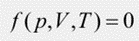
\includegraphics[width=3cm]{img/1.jpeg}
			\caption{Ecuación de estado de un gas ideal. Se evidencian las 	variables de estado.}
			\label{f1}
		\end{figure}

Ahora bien, la ecuación de estado de un gas ideal es aquella que describe el comportamiento de un gas cuando éste se encuentra a una presión baja y a una temperatura alta. En estas condiciones la densidad del gas es muy baja, por lo que pueden decirse que no hay interacciones entre las moléculas del gas y el volumen de las moléculas es nulo.

Además, es el resultado de combinar dos leyes empíricas válidas para gases muy diluidos: la \textbf{ley de Boyle} y la \textbf{ley de Charles}.

\subsection{\textbf{Ley de Boyle}}
	Describe el comportamiento del gas ideal cuando se mantiene su temperatura constante (trasformación isotérmica). Dicha ley establece que el producto de la presión por el volumen de un gas a temperatura constante es constante (k). 
	\begin{figure}[!h]
				\center
				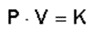
\includegraphics[width=3cm]{img/2.jpeg}
				\caption{Ley de Boyle}
				\label{f2}
	\end{figure}

\subsection{\textbf{Ley de Charles}}
	Establece que, a presión constante, el cociente entre el volumen que ocupa un gas y su temperatura, expresada en kelvin (K), es una constante. 
	\begin{figure}[!h]
				\center
				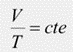
\includegraphics[width=2.5cm]{img/3.jpeg}
				\caption{Ley de Charles}
				\label{f3}
	\end{figure}
	
Combinando las dos ecuaciones tenemos que: 
\begin{figure}[!h]
				\center
				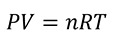
\includegraphics[width=3cm]{img/4.jpeg}
				\caption{Ecuación de estado de un gas ideal}
				\label{f4}
	\end{figure}
	\vspace{30mm}

En donde 
\begin{itemize}
		\item P= presión absoluta
		\item V = volumen
		\item n = número de moles 
		\item constante universal de gas = 8.3145 J/mol K 
		\item T = temperatura 
	\end{itemize}

\subsection{\textbf{Proceso Isotérmico}}
Se le denomina al cambio reversible en un sistema termodinámico, siendo dicho cambio a temperatura constante en todo el sistema. La compresión o expansión de un gas ideal puede llevarse a cabo colocando el gas en contacto térmico con otro sistema de Capacidad calorífica muy grande y a la misma temperatura que el gas; este otro sistema se conoce como foco calórico. De esta manera, el calor se transfiere muy lentamente, permitiendo que el gas se expanda realizando trabajo. Como la energía interna de un gas ideal sólo depende de la temperatura y ésta permanece constante en la expansión isoterma, el calor tomado del foco es igual al trabajo realizado por el gas:  

\begin{figure}[!h]
				\center
				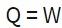
\includegraphics[width=1.8cm]{img/5.jpeg}
				\caption{Calor y trabajo en un proceso Isotérmico}
				\label{f5}
	\end{figure}
	
\subsection{\textbf{Proceso Isocórico }}
Se le denomina al cambio reversible en un sistema termodinámico, siendo dicho cambio a temperatura constante en todo el sistema. La compresión o expansión de un gas ideal puede llevarse a cabo colocando el gas en contacto térmico con otro sistema de Capacidad calorífica muy grande y a la misma temperatura que el gas; este otro sistema se conoce como foco calórico. De esta manera, el calor se transfiere muy lentamente, permitiendo que el gas se expanda realizando trabajo. Como la energía interna de un gas ideal sólo depende de la temperatura y ésta permanece constante en la expansión isoterma, el calor tomado del foco es igual al trabajo realizado por el gas:  

\begin{figure}[!h]
				\center
				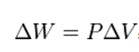
\includegraphics[width=3cm]{img/6.jpeg}
				\caption{Trabajo en un proceso Isocórico}
				\label{f6}
	\end{figure}
	
Aplicando la primera ley de la termodinámica, podemos deducir todo el calor que transfiramos al sistema aumentará a su energía interna U. 
\begin{figure}[!h]
				\center
				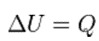
\includegraphics[width=2.3cm]{img/7.jpeg}
				\caption{Energía interna en un proceso Isocórico}
				\label{f7}
	\end{figure}
	
\subsection{\textbf{Proceso Isobárico}}
Es un proceso termodinámico que ocurre a presión constante. La Primera Ley de la Termodinámica, para este caso, queda expresada como sigue:  

\begin{figure}[!h]
				\center
				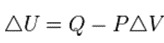
\includegraphics[width=3cm]{img/8.jpeg}
				\caption{Energía interna en un proceso Isobárico}
				\label{f8}
	\end{figure}
%%%%%%%%%%%%%%%%%%%%%%%%%%OBJETIVOS
\section{Objetivos}

	\begin{enumerate}
		\item Comprobar las leyes de los gases 
		\item Entender los diferentes procesos con el gas ideal.
		\item Manejar la ecuación de estado del gas ideal en sus diferentes formas.
		\item Reconocer que el aire en el rango de la temperatura y de presiones trabajadas se comporta como un gas ideal.
	\end{enumerate}
	

%%%%%%%%%%%%%%%%%%%%%%%%%%METODOLOGIA
\section{Metodología}

En el simulador Phet que es el simulador web que nos ayudó en el desarrollo de esta práctica de laboratorio, teníamos una gran variedad de opciones que con el conocimiento previo de los temas que se van a trabajar se puede saber de manera muy intuitiva como es que se configura para evaluar los diferentes procesos, pero enseguida están los pasos:  

\subsection{\textbf{Proceso Isocórico }}
En este, tenemos que seleccionar al volumen como una constante, determinar el tamaño del recipiente que contiene el gas y una cantidad de 100 partículas de las azules. Posteriormente, comenzamos a variar los valores de la temperatura en un total de 10 variaciones para poder crear su respectiva grafica. 

\begin{figure}[!h]
				\center
				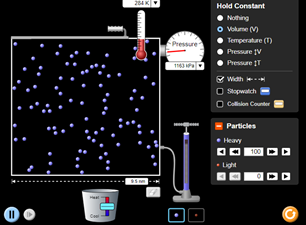
\includegraphics[width=8cm]{img/isoco.png}
				\caption{Configuración utilizada en el simulador Phet a volumen constante}
				\label{f9}
	\end{figure}

\subsection{\textbf{Proceso Isotérmico}}

En este tenemos que seleccionar a la temperatura como una constante, determinar el tamaño del recipiente que contiene el gas y una cantidad de 100 partículas de las azules. Posteriormente, comenzamos a variar los valores del tamaño del recipiente en un total de 10 variaciones para poder crear su respectiva grafica. 
\begin{figure}[!h]
				\center
				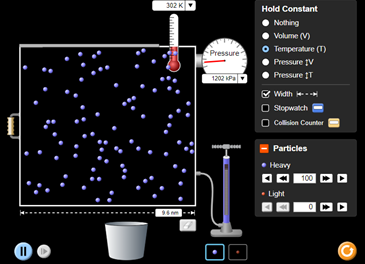
\includegraphics[width=8cm]{img/isote.png}
				\caption{Configuración utilizada en el simulador Phet a volumen constante}
				\label{f10}
	\end{figure}


\subsection{\textbf{Proceso Isobárico}}
En este tenemos que seleccionar a la presión como una constante, determinar el tamaño del recipiente que contiene el gas y una cantidad de 100 partículas de las azules. Posteriormente, comenzamos a variar los valores del tamaño del contenedor del gas en un total de 10 variaciones para poder crear su respectiva gráfica, en este caso podíamos ver que al cambiar el tamaño del recipiente con presión constante la temperatura varia. 

\begin{figure}[!h]
				\center
				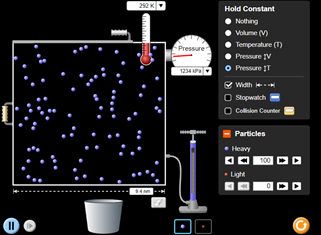
\includegraphics[width=8cm]{img/isoba1.png}
				\caption{A presión constante, se varía el volumen y se registra la temperatura}
				\label{f11}
	\end{figure}
	
	
	A continuación, repetíamos el proceso, pero esta vez con la opción de la presión constante y el volumen, donde en este caso teníamos que elevar o disminuir la temperatura y registrar el tamaño del recipiente puesto que la presión es una constante también. 
	
	\begin{figure}[!h]
				\center
				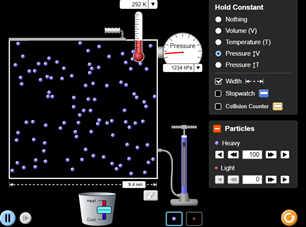
\includegraphics[width=8cm]{img/isoba2.png}
				\caption{A presión constante, se varía la temperatura y se registra el volumen}
				\label{f12}
	\end{figure}
	
	
%%%%%%%%%%%%%%%%%%%%%%%%%%RESULTADOS
\section{Resultados} 

\subsection{Experimento 1: VOLUMEN CONSTANTE}

La ley de Gay Lussac establece que, para un volumen constante de un gas ideal, su presión es directamente proporcional a su temperatura. Si hacemos la gráfica de presión en función de la temperatura, deberíamos ver una línea recta con pendiente positiva, la cual corta o intercepta al eje de la presión (eje Y) en un valor positivo y al ser extrapolada en la temperatura negativa (eje X) , deberíamos encontrar que a una presión de cero (0), la temperatura en kelvin debería ser cercana al cero absoluto o –273.15°C .  

\begin{figure}[!h]
				\center
				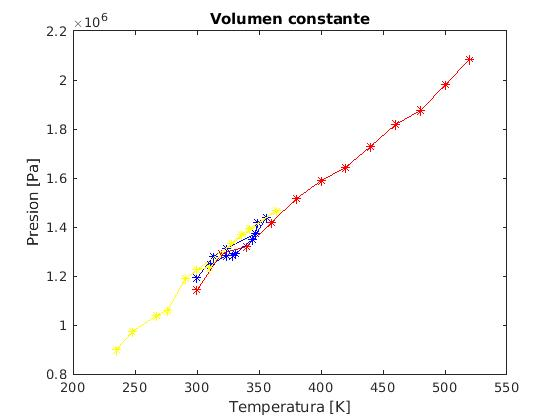
\includegraphics[width=8cm]{img/volcte1.jpg}
				\caption{----}
				\label{f13}
	\end{figure}
	\begin{figure}[!h]
				\center
				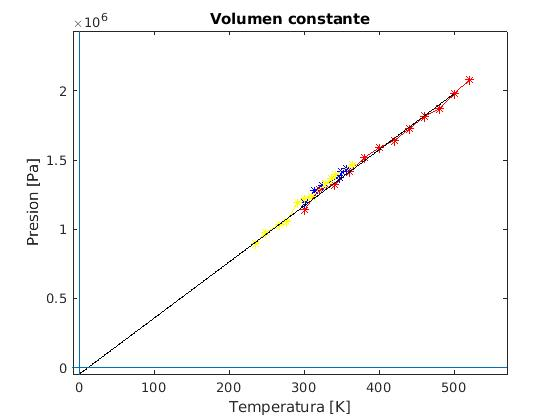
\includegraphics[width=8cm]{img/volcte2.jpg}
				\caption{----}
				\label{f13}
	\end{figure}


\subsection{Experimento 2: TEMPERATURA CONSTANTE}

La ley de Boyle-Mariotte es una ley de los gases que relaciona el volumen y la presión de una cierta cantidad de gas a temperatura constante. Al realizar la gráfica del Volumen en función de la presión esperamos ver una curva, que represente una isoterma, es decir la relación entre presión y volumen a una temperatura constante.  

\begin{figure}[!h]
				\center
				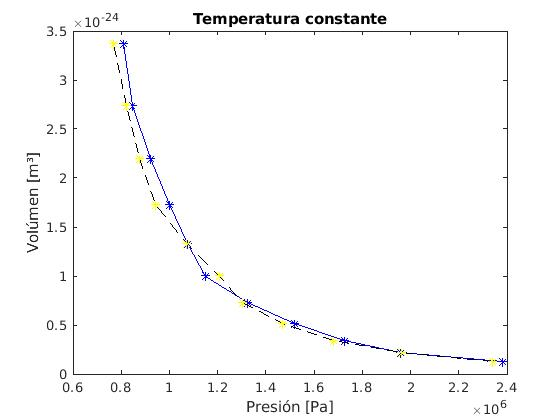
\includegraphics[width=8cm]{img/temcte.jpg}
				\caption{----}
				\label{f14}
	\end{figure}

\subsection{Experimento 3: PRESIÓN CONSTANTE }

La ley de Charles relaciona el volumen y la temperatura de una cierta cantidad de gas ideal, manteniendo la presión constante, la relación es directamente proporcional. Es decir que, al hacer una gráfica del volumen en función de la temperatura, esperamos ver una recta con pendiente positiva. 

Hay dos formas de mantener la presión constante en este sistema. La primera es cambiando el volumen del gas, lo que provocara un efecto en la temperatura para mantener la presión constante. 

\begin{figure}[!h]
				\center
				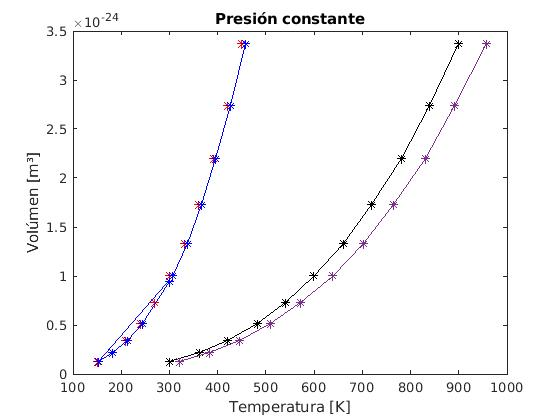
\includegraphics[width=8cm]{img/precte1.jpg}
				\caption{----}
				\label{f15}
	\end{figure}
	
	La segunda forma es variar la temperatura del gas para que el volumen responda de forma proporcional, con el fin de mantener la presión constante.  
\begin{figure}[!h]
				\center
				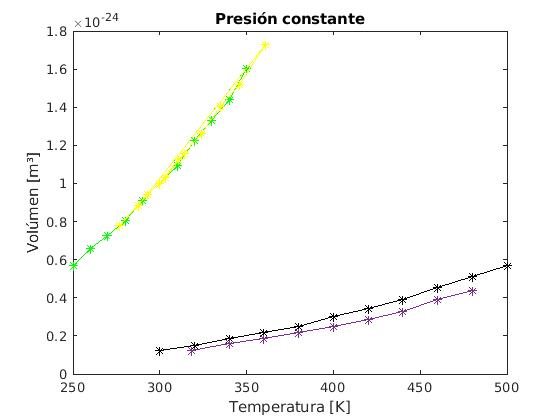
\includegraphics[width=8cm]{img/precte2.jpg}
				\caption{----}
				\label{f16}
	\end{figure}
%%%%%%%%%%%%%%%%%%%%%%%%%%%%%%%%%%%%%%%%%%%%%%%%%%%%RESULTADOS

\section{Análisis de resultados}



\section{Conclusión}
	
	\begin{enumerate}[label=(\roman*)]
		\item Se pudo determinar la relación que existe entre las variaciones y constantes realizada entre la presión, temperatura o volumen, con respecto a las tres leyes de los gases correspondientes a la ley de Gay Lussac, ley de Boyle-Marriotte y ley de Charles.  
		\item  Calculamos la capacidad calorífica de un calorímetro utilizando la técnica de ponerlo en contacto con un elemento de temperatura y masa conocidas para determinar la temperatura de equilibrio de este sistema. 
		\item  Sin importar cuanto calor se le trasmita a un sistema durante un cambio de fase, este no elevará su temperatura, utilizara toda la energía para transformar el elemento del sistema de una fase a otra.
		\item Dos cuerpos en contacto, después de un tiempo, tendrán la misma temperatura.
	\end{enumerate}

\appendices


\ifCLASSOPTIONcaptionsoff
  \newpage
\fi


\begin{thebibliography}{1}


 \bibitem{IEEEhowto:Monteria}
Olmo R. (s.f) Ley de gas ideal [Online]. Recuperado de: http://hyperphysics.phy-astr.gsu.edu/hbasees/Kinetic/idegas.html 

 \bibitem{IEEEhowto:Monteria}
Martín T. y Serrano A. (s.f) Ecuación de estado [Online]. Recuperado de:  https://www2.montes.upm.es/dptos/digfa/cfisica/termo1p/estado.html 
  \bibitem{IEEEhowto:Monteria}
Vidal P. (s.f) Leyes generales de los gases [Online]. Recuperado de:$ https://www.liceopablonerudatemuco.cl/wp-content/uploads/2020/05/QUC38DMICA-8AVO-BC381SICOGuia-leyes-de-Leyes_de_los_gases.pdf $
   \bibitem{IEEEhowto:Monteria}
Katherinne [s.f] Ley de los gases generales [Online]. Recuperado de: https://athanieto.wordpress.com/tematicas/ley-de-los-gases-ideales/ 

\end{thebibliography}



\end{document}